% !TeX program = pdflatex
\documentclass[11pt,a4paper]{article}

\usepackage[margin=2.5cm]{geometry}
\usepackage{amsmath,amssymb}
\usepackage{booktabs}
\usepackage{graphicx}
\graphicspath{{figs/}}
\usepackage{xcolor}
\usepackage[colorlinks=true,allcolors=blue!60!black]{hyperref}
\usepackage{microtype}

\newcommand{\code}[1]{\texttt{\small #1}}
\newcommand{\target}{arXiv:2604.27092}

\title{\bfseries Auditing a claim of autonomous scientific discovery:\\
benchmark integrity, evaluation units, and evidential scope}

\author{Zhengjie Wang\\[2pt]
\small Shanghai Innovation Institute\\
\small \texttt{wangzhengjie@sii.edu.cn}}
\date{\today}

\begin{document}
\maketitle

\begin{abstract}
\noindent
Large language model (LLM) agents are increasingly reported to have
\emph{discovered} scientific results rather than merely to have executed
them. Such attributions are difficult to evaluate: the same artefact---a
working protocol, a measured effect, a manuscript---is produced whether the
agent reasoned its way to a new mechanism or recombined material already
present in its training distribution, retrieved it, or was steered there by a
human. We argue that the discipline currently lacks the minimum reporting and
control standards that would make the distinction decidable, and we propose
five---\textsc{Probe}: \emph{Provenance} disclosure, \emph{Replication} across
independent runs, \emph{Operator-matched} controls, \emph{Benchmark}
integrity, and \emph{Evaluation} pre-registration. We then apply the
checklist to a recent, prominent claim: an LLM agent reported to have
autonomously proposed and experimentally validated a previously unreported
optical mechanism, an ``optical bilinear interaction'' analogous to the
compatibility operation in Transformer attention (\target{}). Working
entirely from the authors' own released data and analysis code, we reproduce
the released benchmark accuracies to within $5\times10^{-4}$ and then show that the
benchmark supporting the computational claim does not survive elementary
integrity checks: the reported cross-split generalisation is accounted for by
the presence of self-paired samples, and the remaining task accuracies are
inflated by near-duplicate repeats shared between training and test folds.
Under ordered-pair-grouped evaluation, pair-identity prediction is not a
well-defined generalisation task, category-pair classification falls below
chance, and same-category classification is not significant under the exact
null distribution over all 105 admissible category assignments
($p=102/105$). In the held-out-category task, above-chance performance occurs
only when self-pairs are present in both the training and the test set;
removing them from either side returns accuracy to chance. We emphasise what
we do \emph{not} claim: we find no evidence in the inspected data that the
measurements were fabricated or internally inconsistent, and the reported
hardware automation may be substantial but is not evaluated by this audit.
The failure is one of evidence--claim alignment within the specific experiment
that carries the computational conclusion.
\end{abstract}

\section{Introduction}
\label{sec:intro}

LLM-based agents have moved, over a short period, from assisting predefined
scientific workflows to being credited with scientific results in their own
right. The claims made on their behalf have escalated accordingly: not that a
system executed a protocol competently, but that it \emph{discovered}
something that was not previously known.

This escalation has outrun the evidence customarily supplied to support it,
for a structural reason. \emph{The artefact produced by genuine discovery and
the artefact produced by retrieval-plus-execution are the same artefact.} An
agent that reasons from physical first principles to a new observable; an
agent that recombines two textbook techniques it has encountered thousands of
times in pretraining; an agent that retrieves a published protocol; and an
agent steered by its operators toward a direction they found promising---all
four emit the same thing at the end. Working code, a measured effect, a
coherent manuscript. Nothing in the output separates them.

For human authorship this problem is bounded, and the bounding is so
thoroughly built into scientific convention that it is easy to forget it is
there. A human author's prior knowledge is finite, largely declarable, and
traceable through citation; the reader can ask what was known and when.
For an LLM agent the prior is a training distribution that is undisclosed,
effectively unbounded, and---in precisely the cases where discovery claims are
most attractive---saturated with the material at issue. Attribution therefore
cannot rest on the output. It has to rest on controls and disclosures that
were never previously required, because they were never previously necessary.

We propose five such requirements (Sec.~\ref{sec:probe}) as a minimal
starting set of reporting and control obligations, and then apply them to a
recent and prominent claim (Secs.~\ref{sec:setup}--\ref{sec:provenance}).
The application is instructive beyond the individual case: two of the failures
we find are invisible to ordinary peer review, because they live in the split
logic and the label construction of a benchmark rather than in any statement
the manuscript makes. They are, however, immediately visible to anyone who
runs the released code with one line changed---which is the argument for
requiring that the code be released, and for looking at it.

We state at the outset what this exercise is not. We allege no misconduct, we
find no evidence of fabrication, and we do not dispute that the automation
demonstrated in the target work is a real achievement.
Section~\ref{sec:caveats} makes the boundaries explicit.

\section{The \textsc{Probe} checklist}
\label{sec:probe}

\paragraph{P --- Provenance disclosure.}
The backbone model and version, its training cut-off relative to the
publication dates of all target papers, the complete initial prompt, every
candidate direction generated and discarded, the criterion by which a
direction was selected and by whom, every human intervention, and the full
agent trace. Without these, the causal attribution ``the agent discovered
$X$'' is not merely unverified but unformulated.

\paragraph{R --- Replication.}
At least three independent runs from the same starting prompt, with the
distribution of outcomes reported. A single trajectory from a stochastic
system cannot distinguish an architectural property from a sampling event.

\paragraph{O --- Operator-matched control.}
Where a physical measurement is claimed to produce information, the control
must be the digital reconstruction of the \emph{same} quantity under the
\emph{same} operator, not a different quantity. Randomising the operator, or
substituting an algebraically distinct expression, tests a different
hypothesis.

\paragraph{B --- Benchmark integrity.}
The evaluation must possess the structure it purports to measure; train/test
partitions must respect the unit of generalisation; and every reported
accuracy must be compared against the best measurement-free rule available on
the same partition, and against an exact or permutation null over the
admissible label assignments where one can be enumerated.

\paragraph{E --- Evaluation pre-registration.}
Readout parameters, feature budgets and splits must be fixed before the
comparison of interest, or the search over them must be reported in full.

\section{Case study: setup}
\label{sec:setup}

The target work couples an LLM multi-agent system to a free-space optical
platform and reports three studies of increasing autonomy, culminating in an
open-ended investigation that identifies an ``optical bilinear interaction''.
Two token-dependent fields $E_a,E_b$ are coherently superposed with controlled
relative phase, scattered by a fixed medium $T$ and detected by a square-law
camera; four-step phase-shifting demodulation with blank subtraction isolates
\begin{equation}
  B_m(a,b) \;=\; E_a^{\dagger}\,\bigl(T_m^{\dagger}T_m\bigr)\,E_b ,
  \label{eq:B}
\end{equation}
a per-channel complex bilinear response. The computational claim is supported
by an eight-token ``semantic benchmark'' comprising 64 ordered pairs and four
tasks: pair identity (A, 64-way), same category (B, binary), category pair
(C, 16-way), and cross-split same-category generalisation to a held-out
category (D).

All material below derives from the authors' own deposit
(DOI \href{https://doi.org/10.5281/zenodo.19890402}{10.5281/zenodo.19890402}).
Our pipeline mirrors
\code{05\_result4\_refine\_paper/scripts/analyze\_advantage\_boundary.py}
so that any difference is attributable to a single documented modification.

\subsection{Replication}
\label{sec:replication}

We first reproduce the released numbers without modification. For the
raw-input baselines---features computed directly from $E(x),E(y)$ with no
optical propagation---the maximum deviation between our values and the
published ones is $5\times10^{-4}$ across all five feature families and all
four tasks. The optical families reproduce likewise, and we independently
recover the authors' participation-ratio effective ranks of the Complex-B
feature ensemble: $3.00$ at $\mathrm{bin}=25$ and $9.62$ at
$\mathrm{bin}=10$, against their stated $\sim$3 and $\sim$9. Nothing that
follows is a pipeline discrepancy.

\section{Benchmark integrity}
\label{sec:benchmark}

\subsection{B1: the benchmark carries no semantic structure}

The eight tokens are constructed as
\begin{verbatim}
def make_token_input(tid):
    seed = 10000 + tid * 7919
    rng  = np.random.default_rng(seed)
    phases = rng.uniform(0, 2*np.pi, (6, 6))
    return np.exp(1j * phases).flatten()      # 36 complex
\end{verbatim}
that is, eight independent unit-modulus random phase vectors. The words
(\emph{cat}, \emph{dog}, \emph{hammer}, \dots) and the categories
(\emph{animals}, \emph{tools}, \dots) are labels attached to random vectors;
no embedding enters the pipeline. Consequently the proposition ``\emph{cat}
and \emph{dog} belong to the same category'' is encoded nowhere in the inputs
or in the physics. The data-generating process contains no designed semantic
relation from which held-out-category generalisation could be learned; any
above-chance Task-D result must therefore be attributed to a finite-sample
accident or to an evaluation cue, rather than to encoded semantics recovered
by the measurement.

\subsection{B2: Task D is accounted for by self-pairs}

For each held-out category the test set contains 4 distinct positive pairs, of
which 2 are self-pairs $(x,x)$, against 24 distinct negatives. The
measurement-free identity-rule baseline
``$\text{same category} := (x=y)$'' therefore attains balanced accuracy
$\tfrac12\bigl(\tfrac24 + \tfrac{24}{24}\bigr) = 0.750$. Every full-readout
value displayed in Fig.~\ref{fig:D} lies at or below this baseline. We do not
extend the comparison either to values reported under the different
fixed-holdout protocol of the main manuscript, or to the higher values the
supplement obtains under searched sparse-tap and output-budget
configurations; those are exactly the configurations whose selection timing
the public record does not document (Sec.~\ref{sec:search}). Removing all
self-paired samples collapses the optical feature to chance
(Fig.~\ref{fig:D}), identically at both readout scales, while the per-fold
values are constant to four decimals in the unablated case---the signature of
a deterministic structural cue rather than a learned relation.

\begin{figure}[t]
\centering
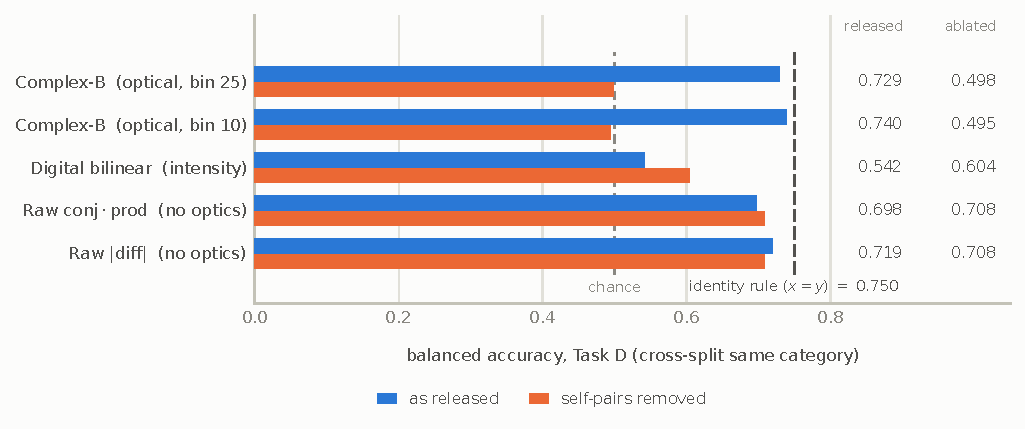
\includegraphics[width=\linewidth]{fig1_taskD_selfpair.pdf}
\caption{\textbf{Task D is accounted for by self-pairs.} Balanced accuracy on
the cross-split same-category task under the refined held-out-category
protocol, before and after removing every self-paired sample $(x,x)$. The
dashed rule at $0.750$ is the accuracy of the measurement-free identity rule
``same category $:=(x=y)$'', which uses the pair labels and no optical data at
all. The optical Complex-B feature does not exceed that rule, and falls to
chance once self-pairs are removed---identically at the coarse
($\mathrm{bin}=25$) and speckle-matched ($\mathrm{bin}=10$) readouts. The
raw-input baselines, which involve no optical propagation whatsoever, are
unaffected by the ablation.}
\label{fig:D}
\end{figure}

\subsection{B3: Tasks A--C are inflated by repeat leakage}

Throughout this subsection, ``leakage'' means leakage relative to a claim of
out-of-pair or semantic generalisation. If the tasks were intended only to ask
whether repeated measurements of an already-observed pair can be recognised,
splitting repeats at random is legitimate; the tasks then simply cannot
support claims about category structure or new pairs.

The released scoring applies \code{StratifiedKFold} over 320 samples
comprising 64 pairs $\times$ 5 physical repeats, so repeats of the same pair
are split between training and test folds. We measure the pairwise repeat
correlation of the Complex-B feature directly: mean $0.9828$, with $97.0\%$ of
repeat pairs exceeding $0.97$ (Fig.~\ref{fig:corr}), confirming the authors'
own figure. Training and test folds thus contain near-duplicates of the same
measurement.

Re-scoring with \code{StratifiedGroupKFold} grouped by ordered pair gives
Table~\ref{tab:ABC} and Fig.~\ref{fig:leak}. Pair identity is not evaluable as
an out-of-pair generalisation task when the ordered pair is the grouping unit,
because each 64-way class corresponds to exactly one group; and Task C falls
to or below the 16-class chance level of $0.0625$. We verified that the Task-C collapse is not
an artefact of the fold count: across $n_{\text{splits}}\in\{2,4,5,8\}$ every
test class is represented in training ($100\%$) and accuracy remains in
$0.043$--$0.109$ at both readouts (Fig.~\ref{fig:leak}c).

\begin{figure}[t]
\centering
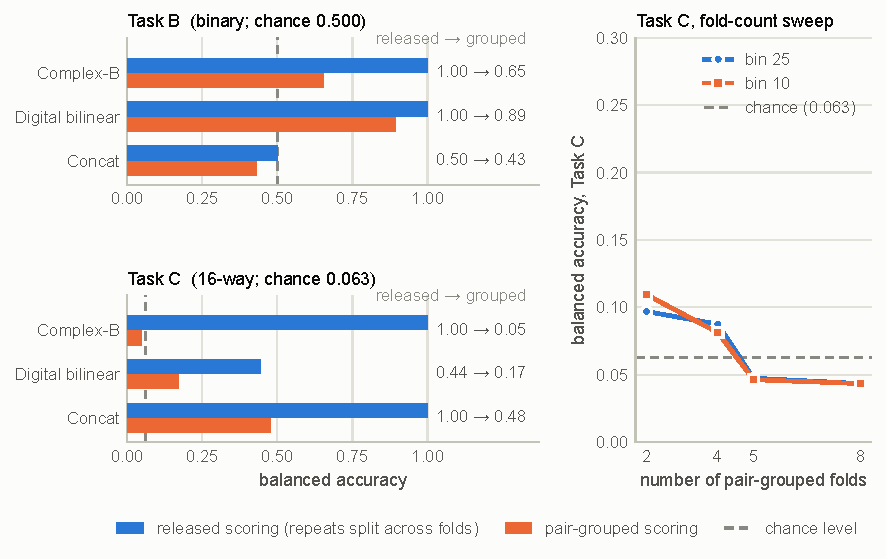
\includegraphics[width=\linewidth]{fig2_leakage.pdf}
\caption{\textbf{Tasks B and C are inflated by repeat leakage.}
(\textbf{a},\textbf{b}) Balanced accuracy at $\mathrm{bin}=25$ under the
released scoring, which splits the five physical repeats of a pair across
folds, and under pair-grouped scoring, which does not. (\textbf{c}) The
Task-C collapse is not a fold-count artefact: it persists across
$n_{\text{splits}}\in\{2,4,5,8\}$ at both readouts, with every test class
represented in training in all cases.}
\label{fig:leak}
\end{figure}

\begin{figure}[t]
\centering
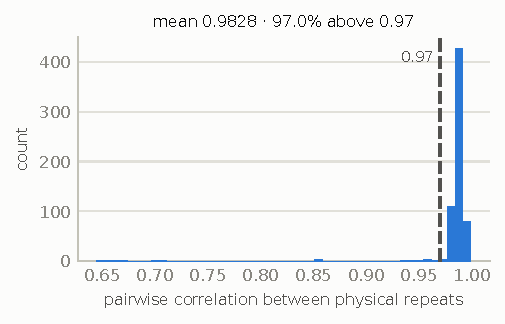
\includegraphics[width=0.56\linewidth]{fig3_repeat_correlation.pdf}
\caption{\textbf{Physical repeats are near-duplicates.} Distribution of
pairwise correlations between the five repeated measurements of the Complex-B
feature, over all 64 ordered pairs at $\mathrm{bin}=25$. Under the released
scoring these near-duplicates are distributed across training and test folds.}
\label{fig:corr}
\end{figure}

\begin{table}[t]
\centering
\caption{Tasks A--C at $\mathrm{bin}=25$, balanced accuracy, released scoring
versus pair-grouped scoring.}
\label{tab:ABC}
\begin{tabular}{llccc}
\toprule
Feature & Task & released & pair-grouped & $\Delta$ \\
\midrule
Complex-B        & A (64-way)  & 1.0000 & \multicolumn{2}{c}{degenerate by construction} \\
Complex-B        & B (binary)  & 1.0000 & 0.6522 & $-0.3478$ \\
Complex-B        & C (16-way)  & 1.0000 & 0.0474 & $-0.9526$ \\
Digital bilinear & B (binary)  & 1.0000 & 0.8917 & $-0.1083$ \\
Digital bilinear & C (16-way)  & 0.4437 & 0.1709 & $-0.2729$ \\
\bottomrule
\end{tabular}
\end{table}

\subsection{B4: the residual Task-B accuracy is not significant}

Pair-grouped scoring leaves Task B at $0.6522$, above the binary chance level.
This residual admits an exact test. The same-category label is fixed entirely
by a partition of the eight tokens into four unlabelled two-token categories,
and there are $8!/((2!)^4 4!) = 105$ such partitions. We therefore recompute
the pair-grouped Task-B accuracy under every admissible assignment. The
designated semantic assignment is a member of this set, so the exact one-sided
$p$-value is the fraction of assignments scoring at least as high as the
designated one, with the designated assignment counted in the numerator; no
Monte Carlo sampling and no continuity correction are involved.

The designated assignment scores $0.6522$ against a null with mean $0.7280$
and standard deviation $0.0347$, and $102$ of the $105$ assignments score at
least as high (Fig.~\ref{fig:perm}); the exact one-sided $p$ is $0.9714$.
Approximately $97\%$ of all admissible category assignments therefore achieve
accuracy at least as high as the designated semantic one. The residual is not
evidence that the measurement recovers the designated category structure.

\begin{figure}[t]
\centering
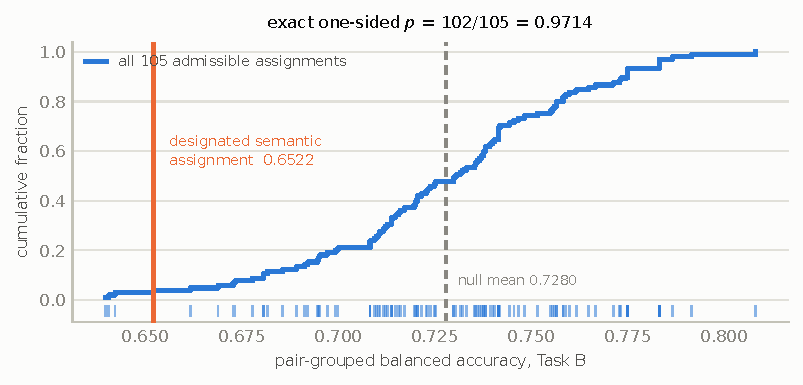
\includegraphics[width=0.80\linewidth]{fig4_permutation_null.pdf}
\caption{\textbf{The residual Task-B accuracy is not exceptional.} Empirical
cumulative distribution and rug plot of pair-grouped Task-B balanced accuracy
over \emph{all} 105 partitions of the eight tokens into four unlabelled
two-token categories---an exact enumeration, not a Monte Carlo sample. The
designated semantic assignment lies in the lower tail.}
\label{fig:perm}
\end{figure}

\subsection{B5: the Task-D shortcut is learned, not merely present}

Removing self-pairs from the training set and from the test set are distinct
interventions, and crossing them separates a cue that the classifier acquires
during fitting from a structural shortcut sitting in the test set.
Table~\ref{tab:2x2} gives the full design. Above-chance performance occurs
only when self-pairs are present on \emph{both} sides; removing them from
either side returns accuracy to chance. In particular, when self-pairs are
present at test time but absent during training, accuracy is $0.4917$---the
shortcut is available but unused. This is a learned self-pair shortcut under
this evaluation protocol. We note the small effective sample: each held-out
fold contributes only 4 distinct positive pairs (2 after ablation) against 24
distinct negatives.

\begin{table}[t]
\centering
\caption{Task D at $\mathrm{bin}=25$ under the full $2\times2$ self-pair
design. Identical classifier, folds and scoring throughout.}
\label{tab:2x2}
\begin{tabular}{llcc}
\toprule
Self-pairs in training & Self-pairs in test & balanced accuracy & test $+$/$-$ \\
\midrule
present & present & 0.7292 & 20 / 120 \\
present & removed & 0.4792 & 10 / 120 \\
removed & present & 0.4917 & 20 / 120 \\
removed & removed & 0.4979 & 10 / 120 \\
\bottomrule
\end{tabular}
\end{table}

\section{Model--measurement consistency: a diagnostic observation}
\label{sec:ideal}

This section is diagnostic rather than evaluative. It bears on neither the
benchmark failures of Sec.~\ref{sec:benchmark} nor the central attribution
question, and we report it because it constrains what the released estimator
can be assumed to satisfy.

Under the stated linear-optical model the unbinned channel kernel
$K_p = T_p^{\dagger}T_p$ is \emph{algebraically} rank-one, Hermitian and
positive semidefinite; spatial binning forms $K_k=\sum_{p\in\mathcal{B}_k}K_p$,
a positive semidefinite sum whose algebraic rank is bounded by the number of
independent propagation rows in the bin. These are consequences of the model,
not empirical assumptions, and they imply $B_p(y,x)=B_p(x,y)^{\ast}$.

What the release contains is an estimator carrying a reference arm, phase
stepping, blank subtraction, drift and calibration error. It satisfies the
ideal identities only approximately. Over the 28 off-diagonal token pairs the
mean correlation between $\widehat B(y,x)$ and $\overline{\widehat B(x,y)}$ is
$0.6042$, against $0.1537$ for the uncorrelated comparison $\widehat B(x,y)$;
the conjugate symmetry is thus clearly present but far from exact. On
self-pairs, where the model predicts a positive real value, the real part is
non-negative in every channel, but the mean relative imaginary magnitude
$|\mathrm{Im}\,\widehat B|/|\widehat B|$ is $0.3511$.

A phase-gauge offset would reproduce this signature without implying that the
cross term was not isolated, so we tested it: estimating a single global phase,
and then a per-channel phase, from the self-pairs alone and applying it to all
pairs. Neither accounts for the departure. The self-pair imaginary ratio falls
only from $0.3511$ to $0.3102$ (global) and $0.3057$ (per-channel), and the
swap-conjugate correlation does not improve ($0.5666$ and $0.5606$). The
per-channel phases are moreover nearly identical (circular spread $0.0019$), so
there is no channel-dependent phase structure to remove.

We draw no conclusion about the cause. Two candidate explanations remain open
and are not separable from the released data: a residual in the blank or
reference subtraction, and the two input arms not sharing a transmission
operator, $T_x \neq T_y$. We flag that the second would also weaken one line
of criticism available against the attention analogy, since a kernel
$T_x^{\dagger}T_y$ is rank-one but neither Hermitian nor positive
semidefinite, and is in that respect \emph{less} constrained than the
shared-operator case. Resolving this requires acquisition-level information
that the deposit does not contain.

\section{The missing operator-matched control}
\label{sec:operator}

Equation~\eqref{eq:B} is the cross term of two-beam interference, isolated by
four-step phase shifting. Under linear optics the jointly demodulated field
and the digital product $A_x^{\ast}\!\odot A_y$ of the separately measured
complex output fields $A_x, A_y$ are the same quantity up to noise. The
decisive control is therefore an equality test between the jointly demodulated
field and that digital product, formed from the fields the \emph{actual} two
arms produce. We deliberately do not phrase this as a shared-$T$ test: as
Sec.~\ref{sec:ideal} shows, the released estimator does not closely satisfy
the shared-operator identities, so $A_x=T_xE_x$ and $A_y=T_yE_y$ with
$T_x\neq T_y$ must be admitted. The shared-operator case is a special
instance, not the general requirement.

The released controls are not this test. The ``digital bilinear'' baseline is
$z(x)\,z(y)$ where $z$ is binned camera \emph{intensity}, discarding phase;
a further variant is described in the supplement as a per-channel product
``no cross-conjugation''; and the pseudo-$B$ control replaces the physical $T$
with a random complex Gaussian. The first two compare different algebraic
objects; the third asks whether a real scattering matrix differs from a random
one, not whether joint measurement yields information unavailable to separate
measurement. The required control is absent, and---because this experiment
records only single-token \emph{intensity}---it cannot be performed on the
released data. It can, however, be performed on the same apparatus: the
self-referenced transmission-matrix measurement in the earlier studies of the
same work recovers exactly the complex fields it requires.

\section{What is, and is not, implemented relative to attention}
\label{sec:attention}

The manuscript describes the measured quantity as structurally analogous to a
core operation in Transformer attention. We set out precisely how far that
correspondence extends, because the claim is otherwise easy to read as
stronger than the experiment supports.

An attention compatibility score is
\begin{equation}
  s(x,y) \;=\; x^{\top} W_Q^{\top} W_K\, y ,
\end{equation}
while a measured detector channel supplies
\begin{equation}
  B_k(x,y) \;=\; x^{\dagger} K_k\, y .
\end{equation}
Both are two-input bilinear (respectively sesquilinear) compatibility forms,
so the stated analogy holds in that weak mathematical sense, and we do not
dispute it at that level.

The differences are the substance. $W_Q$ and $W_K$ are learned, may be
distinct, and their product is a general matrix; $K_k$ is fixed by the medium
and is not adjustable at all. Under the ideal shared-operator model each
unbinned $K_p$ is a rank-one positive semidefinite outer product and a binned
$K_k$ is a finite sum of such terms, so the realisable operator family is a
restricted subclass rather than a general learnable bilinear map---though, as
Sec.~\ref{sec:ideal} notes, if the two arms do not share an operator this
particular restriction is weaker than it appears. Beyond the operator itself,
the experiment does not construct a token-pair score matrix, and it implements
no scaling, no softmax normalisation, no masking, no value projection and no
value aggregation. No end-to-end attention task is run, and the readout is a
linear classifier applied digitally to the measured features.

The defensible reading is therefore that the experiment demonstrates a
restricted physical pair-feature primitive, not an implementation of
Transformer attention and not attention hardware.

\section{Evaluation search space}
\label{sec:search}

The evaluation supporting the computational claim involves several free
choices, and the released material shows that more than one value of most of
them was examined. Table~\ref{tab:search} records the search space that is
publicly visible, alongside what the public record does and does not establish
about when each choice was fixed. We stress the distinction: for none of these
choices do the released materials document the selection \emph{timing}, and we
therefore do not assert that any of them was made after inspecting the
outcome. What the record does establish is that the reported configuration was
selected from a searched space without an independent confirmation set. This
is adaptive evaluation, and the standard remedy---pre-registration of the
readout parameters and splits, or a held-out physical realisation on which the
selected configuration is evaluated once---was not applied.

\begin{table}[t]
\centering\small
\caption{Publicly visible evaluation search space for the Result-4 benchmark.}
\label{tab:search}
\begin{tabular}{p{3.0cm}p{4.0cm}p{3.4cm}p{2.6cm}}
\toprule
Choice & Publicly observed search & Selection timing & Independent confirmation \\
\midrule
Detector bin & 5, 10, 25 & Not publicly documented & None identified \\
Output budget & multiple $n_{\text{out}}$ values & Not publicly documented & None identified \\
Task-D protocol & multiple descriptions and implementations & Protocol evolution observed & None identified \\
Feature family & multiple optical and digital families & Exploratory analysis evident & None identified \\
Token vocabulary & one fixed random codebook & Not publicly documented & No independent vocabulary \\
\bottomrule
\end{tabular}
\end{table}

\section{Provenance}
\label{sec:provenance}

The central claim is causal: that an agent, rather than its training
distribution or its operators, originated the mechanism. Searching the full
deposit we find no backbone model name or version, no system or initial
prompts, no agent trace, no record of human intervention, and no
direction-selection log; the deposit states explicitly that the engine and
hardware-control software are not included. What is released---result-level
data and offline analysis scripts---establishes that the numbers can be
recomputed. It cannot establish where the idea came from.

We note a further tension internal to the released material. The staged
reports characterise the contribution in measured terms: phase-stepping
interferometry is ``a mature technique'', and ``the methodological novelty is
not the demodulation itself but its application to extract a computationally
meaningful bilinear observable''. The abstract of the manuscript describes the
same object as a ``previously unreported physical mechanism''. We record this
as an internal inconsistency in how the contribution is characterised. It is
not a completed novelty audit: establishing that the physical claim is
overstated would require a systematic prior-art search over phase-shifting
interferometry, coherent and heterodyne detection, optical and joint-transform
correlators, coherent optical multiplication, complex-field inner-product
measurement, photonic bilinear computing and scattering-medium random
features, which we have not carried out. Our position is that physical
novelty is \emph{not established} by the released materials, not that it is
absent.

\subsection{Architectural attribution}

A separate attribution problem sits beneath the provenance one, and survives
even if the trajectory were accepted as fully autonomous. The manuscript
credits specific architectural components---Meta-Trace, the dual-layer
separation, role--phase decoupling, accumulated research experience---with
sustaining the long-horizon trajectory. A single successful run cannot
identify which component, if any, produced the outcome. The released material
contains no single-agent baseline, no run with Meta-Trace replaced by ordinary
rolling summarisation, no fixed-workflow comparison, no ablation of the
Critical Reviewer role, no run without inherited prior-study experience, no
variation of random seed, and no variation of backbone model. Nor is there a
human-expert time or cost baseline against which the reported speed advantage
could be assessed. The reported totals---145.9 million tokens, 3{,}242 model
calls, 1{,}242 tool invocations---are resource counts. They record what was
spent, not which architectural choice was responsible for what was obtained.

\section{Discussion}
\label{sec:discussion}

\subsection{Limits of the computational interpretation}

\paragraph{Scale and effective dimensionality.}
The released computational demonstration contains eight fixed tokens and
64 ordered pairs, all derived from one deterministic random-phase codebook.
It therefore does not test generalisation to a larger vocabulary, to newly
encoded tokens, to another random codebook, or to an independently acquired
physical operator. The target work itself identifies vocabulary scale as a
limitation and notes, in the authors' released Report 4, that a related
token-family representation previously exhibited degeneracy-boundary collapse
at $N=16$.

Nominal detector dimensionality should also be distinguished from effective
dimensionality on the evaluated data. At the main-text bin size of 25 pixels,
we reproduce a participation-ratio effective rank of 3.00 for the released
Complex-B feature ensemble, despite hundreds of nominal detector channels;
at bin size 10 the corresponding value is 9.62. These quantities are
properties of the observed eight-token feature ensemble, not universal rank
bounds on the apparatus. They nevertheless show that the high-dimensional
capacity invoked in the computational interpretation was not demonstrated on
the benchmark used to support it: most observed variation is concentrated in
a small number of effective complex directions, and near-saturated accuracy
is obtained on a correspondingly small, repeatedly observed vocabulary.

\paragraph{Speed and energy are unmeasured outlooks.}
The experiment establishes that the complex cross term can be recovered on
the physical platform; it does not establish a system-level speed or energy
advantage. In the released acquisition protocol, each ordered input pair is
measured through four sequential phase settings. The overall protocol also
contains blank-control measurements, camera readout, calibration,
normalisation, demodulation, and digital classification. Blank controls may
be reused across multiple pairs and therefore should not automatically be
counted as a per-pair cost, but they remain part of the demonstrated system.

No end-to-end latency, pair-score throughput, energy per recovered score,
total system power, or amortised calibration cost is reported in the public
materials. Nor is the demonstrated implementation compared under a matched
accuracy and precision target with a GPU, FPGA, or digital complex
correlator. The current experiment acquires the ordered pairs individually;
it does not demonstrate parallel construction of an $N\times N$ score
matrix, softmax normalisation, value projection, or value aggregation.
Future spatial, wavelength, or temporal parallelisation may change this
assessment, but it is not measured here. Statements concerning high-speed or
energy-efficient Transformer-like hardware should therefore be read as
prospective motivation rather than experimental findings of the present
study.

\paragraph{Protocol evolution and confirmatory status.}
The released reports document an evolving analysis rather than one fixed
confirmatory protocol. Report 4 and Report 5 describe different
cross-split constructions and report materially different behaviour across
feature families. The later analysis additionally explores detector bin
sizes, output-channel budgets, sparse-tap selections, raw-input controls,
random-operator controls, and revised task definitions. Such exploration is
scientifically useful and, when reported transparently, is not itself an
error. Because the documented Task-D protocols are not identical, we do not
treat numerical differences between the two reports as controlled
method-to-method comparisons.

It does, however, change the evidential status of the resulting performance
comparisons. The public materials do not document when the token vocabulary,
task definitions, split rules, bin size, output budget, or highlighted
operating point were fixed relative to inspection of the corresponding
outcomes. No independently acquired confirmation set or new physical
operator is used after these choices. We therefore interpret the released
performance landscape as exploratory. A confirmatory computational claim
would require a frozen protocol evaluated on new tokens, a new codebook, an
independent acquisition, or another physical realisation without further
selection of readout configuration.

\section{Scope and unaudited claims}
\label{sec:scope}

This audit is deliberately claim-specific. We examine the released Result-4
pipeline because it provides the empirical basis for the manuscript's claims
concerning optical bilinear computation, semantic pair representation, and the
analogy to a core operation in Transformer attention. We reproduce and
stress-test the public data, scripts, feature construction and evaluation
protocol associated with that result.

We do not present a complete audit of the two preceding studies. In
particular, we have not independently evaluated the optical acquisition
efficiency or the focusing-enhancement deficit in the transmission-matrix
reproduction (Result 2), nor have we reconstructed the full
theory-to-measurement argument, mixed-state synthesis or uncertainty
propagation in the majorization-order study (Result 3). We therefore draw no
conclusion about the correctness, novelty or autonomy of those results. Their
inclusion in the target manuscript does not, however, resolve the
benchmark-integrity failures identified for Result 4, nor does it provide
evidence for the specific computational claims tested here.

Our operator analysis is similarly bounded. We distinguish identities that
follow from the ideal shared-operator model from properties of the released
experimental estimator. The empirical deviations reported in
Sec.~\ref{sec:ideal} do not identify their physical cause. They may arise from
unequal propagation operators in the two input arms, residual self-reference
terms, imperfect phase stepping, calibration error, drift, or another
unmodelled component. Resolving these alternatives requires measurements and
hardware information not present in the public deposit.

Finally, statements about absent evidence refer only to the public record
available to us as of 30 July 2026: arXiv:2604.27092v1 and the Zenodo deposit
10.5281/zenodo.19890402. The deposit states that the formal Supplementary
Information submitted to the journal, the Qiushi Engine core system and the
hardware-control software are not included. We therefore distinguish ``not
present in the public materials'' from ``not performed''. In particular, we
cannot determine whether an operator-matched reconstruction, additional
agent-provenance records or alternative evaluation protocols exist in
non-public submission materials.

\section{What we do not claim}
\label{sec:caveats}

We find no evidence in the inspected Result-4 data that the hardware
measurements were fabricated or internally inconsistent. The raw frames,
repeat structure and drift monitoring are substantial and mutually consistent.
We make no assessment of the reported hardware automation---sustained agent
control of a real optical platform over hundreds of steps---because the
materials required to evaluate it are not public and we did not audit it; our
findings neither support nor challenge it. Our claim is narrower and, we
think, more serious: the specific evidence offered for the specific central
computational conclusion does not support it.

\section{Evidence needed to adjudicate the claims}
\label{sec:settle}

The deficiencies identified above are resolvable. They require different
evidence for the computational, physical, and autonomy claims; no single
additional accuracy value would address all three.

\paragraph{Agent provenance.}
Attribution of an idea to an autonomous agent requires disclosure of the
backbone model and exact version, inference settings, initial and system
prompts, retrieval sources, progressively disclosed skills, candidate
directions, direction-selection decisions, and human interventions. The
complete time-ordered Meta-Trace and tool trajectory should be released in a
form that distinguishes contemporaneous records from summaries produced
after the experiment. If safety, licensing, or instrument-access constraints
prevent release of particular implementation details, the omitted fields and
their relevance to the claimed discovery should be identified explicitly.
Result-level data alone cannot establish the causal origin of the hypothesis.

\paragraph{Prior-availability control.}
The relevant question is not whether a current language model can reproduce
the mechanism after publication, but whether the backbone available to the
agent before the study already contained or could readily elicit the same
proposal. This should be tested using the exact original model snapshot,
without the agent scaffold or experimental feedback, from the same initial
platform description. The prompt, decoding parameters, number of independent
queries, retrieval permissions, and a prospectively defined scoring rule
should be fixed before inspection of the outputs. The assessment should
separately record whether the model proposes the interference cross term and
whether it identifies the underlying phase-stepping and coherent-detection
principles as established knowledge. Such a control would measure prior
availability; it would not by itself prove the causal origin of the observed
trajectory.

\paragraph{Operator-matched physical control.}
For each detector pixel, the ideal shared-operator model predicts
\begin{equation}
 B_p(x,y)=(TE_x)_p^{*}(TE_y)_p .
\end{equation}
For a binned channel $\mathcal{B}_k$, the corresponding reconstruction is
\begin{equation}
 \bar B_k^{\mathrm{digital}}(x,y)
 =
 \sum_{p\in\mathcal{B}_k}
 (TE_x)_p^{*}(TE_y)_p .
\end{equation}
The decisive control is therefore to measure the two propagated complex
fields separately under the same physical operator and compare this digital
reconstruction, channel by channel, with the jointly demodulated
$\bar B_k^{\mathrm{physical}}$. Agreement should be quantified in amplitude,
phase, residual structure, repeatability, and downstream performance under
identical feature budgets and splits. If the two input arms implement
different operators, the corresponding $T_x^{\dagger}T_y$ model should be
stated and tested instead. This experiment would determine whether joint
measurement supplies information beyond separately measured complex fields;
intensity products and random-operator pseudo-$B$ controls do not answer that
question.

\paragraph{Benchmark with a valid unit of generalisation.}
A confirmatory benchmark should contain relational structure in the inputs
rather than attach semantic labels to independent random vectors. It should
use tokens, codebooks, or physical inputs not involved in configuration
selection. All repeated measurements of the same physical condition must
remain in the same fold whenever the claim concerns generalisation to new
conditions. Self-pairs should either be excluded from relation evaluation or
reported as a separate stratum, and performance should be compared with
measurement-free structural rules and an exact or permutation null over
admissible label assignments. Pair identity may be evaluated as repeat
recognition, but it should not be interpreted as out-of-pair generalisation.
The final test should use a new acquisition session, codebook, vocabulary, or
physical operator after the evaluation protocol has been frozen.

\paragraph{Independent agent and hardware replications.}
A single successful trajectory cannot establish that the reported outcome is
a reproducible property of the agent architecture. The open-ended study
should be repeated independently from the same initial information, with all
runs and unsuccessful directions retained. At least three complete runs would
provide a minimal existence check, although more are required to estimate a
meaningful discovery rate for a stochastic system. Replication should also
separate agent stochasticity from hardware specificity by including, where
feasible, an independent acquisition session or physical realisation. The
reported outcomes should include the frequency with which the mechanism is
proposed, selected, experimentally supported, rejected, or replaced by
another direction.

\paragraph{Pre-registered confirmation.}
Before the confirmatory run, the token set, task definitions, train--test
unit, treatment of self-pairs, detector binning, output budget, feature
families, classifier, hyperparameters, primary endpoint, and statistical
comparison should be frozen in a time-stamped protocol. Exploratory searches
over bin size, $n_{\mathrm{out}}$, task construction, or feature family may be
reported in full, but the selected configuration should then be evaluated on
untouched data without further adaptation. This separation would turn the
released performance landscape from an exploratory result into a test of a
specified computational claim.

Together, these additions would not require treating autonomous discovery as
a binary label. They would allow readers to distinguish four progressively
stronger conclusions: automated execution of a known protocol, recombination
of available scientific knowledge, generation and testing of a new
engineering interpretation, and experimental identification of a finding
not available to the model or its operators beforehand.

\section*{Data and code availability}
All analysis code, the audit modifications and the full result files are at
\url{https://github.com/[user]/discovery-audit}. The audit consumes only the
authors' public deposit (DOI 10.5281/zenodo.19890402); no data of our own were
generated, and the deposit is not redistributed. Every file read from the
deposit is recorded with its SHA-256 in \code{results/input\_manifest.json};
the roll-up digest over all 1543 consumed files is
\code{b273f7f6c8d5bd8d7bb849e1d9908ea35a8ec171b9870b7cd2cb27b496351350}, so any
subsequent change to the deposit is detectable. The environment is pinned in
\code{environment.yml} and \code{requirements-lock.txt}.

\begin{thebibliography}{9}\small
\bibitem{qiushi} S.~Yang \emph{et al.},
  \emph{End-to-end autonomous scientific discovery on a real optical
  platform}, arXiv:2604.27092 (2026).
\bibitem{zenodo} S.~Yang, Source materials, DOI 10.5281/zenodo.19890402 (2026).
\bibitem{popoff} S.~M.~Popoff \emph{et al.},
  \emph{Measuring the transmission matrix in optics}, Phys.\ Rev.\ Lett.\
  \textbf{104}, 100601 (2010).
\bibitem{hamerly} R.~Hamerly \emph{et al.},
  \emph{Large-scale optical neural networks based on photoelectric
  multiplication}, Phys.\ Rev.\ X \textbf{9}, 021032 (2019).
\bibitem{attention} A.~Vaswani \emph{et al.},
  \emph{Attention is all you need}, NeurIPS \textbf{30} (2017).
\end{thebibliography}

\end{document}
